\documentclass[a4paper,12pt]{article}
\usepackage[utf8]{inputenc}
\usepackage[T1]{fontenc}
\usepackage{amsmath}
\usepackage{amsfonts}
\usepackage{amssymb}
\usepackage{geometry}
\geometry{margin=1in}
\usepackage{xcolor}
\usepackage{graphicx}
\usepackage{enumitem}   
\usepackage{url}
\usepackage{hyperref}
\usepackage[most]{tcolorbox}
\usepackage{parskip}  % Remplace les indentations par des sauts de ligne
\usepackage{amsmath}% pour l’option [label=(…)]


\title{CONSTANTE D'EULER-MASCHERONI \(\gamma\)
Qassemyar David ;
    Berthomé Baptiste ;
    Adabadji-Parriel Kossi-Félicité ;
    Randrianarisoa Mendrika-Kamel}
\begin{document}

\author{}
\date{}

\maketitle
\begingroup 
\Large
\tableofcontents
\endgroup 

\newpage
\section*{Introduction}


La constante d'Euler-Mascheroni, notée $\gamma$, définie par :

\begin{tcolorbox}[colback=blue!5!white,colframe=blue!75!black$\gamma$]
\[
\gamma = \lim_{n \to +\infty} \left( \sum_{k=1}^n \frac{1}{k} - \ln n \right)
\]
\end{tcolorbox}\\
reste l'une des constantes les plus énigmatiques des mathématiques modernes. Découverte au XVIII\textsuperscript{e} siècle, elle résiste encore aujourd'hui aux questions les plus fondamentales sur sa nature arithmétique -- son irrationalité n'est toujours pas démontrée, et sa transcendance demeure un mystère complet. Le célèbre mathématicien G.H. Hardy alla jusqu'à promettre sa chaire à Oxford pour qui prouverait l'irrationalité de $\gamma$, témoignant de l'importance du problème. \\

Dès sa première évaluation par Euler ($0{,}577\,218$ en 1735), cette constante a suscité un intérêt croissant. Mascheroni, Gauss, puis John Couch Adams repoussèrent successivement les limites du calcul numérique, atteignant respectivement 32, 22 et 263 décimales. L'avènement de l'informatique permit ensuite à John William Wrench d'établir 328 décimales en 1952 -- un record qui ne fit qu'augmenter avec les supercalculateurs modernes. \\

Apparue initialement dans l'étude des séries harmoniques, $\gamma$ s'est révélée omniprésente en mathématiques :
\begin{itemize}
    \item En analyse, via les fonctions $\Gamma$ et $\psi$

    \item En théorie des nombres, liée à la fonction zêta
    \item En probabilités, dans la loi de Gumbel
    \item En algorithmique, où son calcul pose des défis numériques
\end{itemize} \\

Malgré toutes ces apparitions dans de nombreux domaines variés, $\gamma$ conserve ses secrets les plus profonds, faisant d'elle l'une des constantes les plus fascinantes de l'analyse moderne, considérée comme la troisième constante mathématique la plus importante après $\pi$ et e.

\newpage

\section{Démonstrations de l'existence et approximations de $\gamma$}

\subsection{Théorème de la limite monotone }
    
    \textbf{Théorème 1 : } $\[\gamma = \lim_{n \to \infty} \left( H_n(n) - ln(n) \right)\]$ \\
    
    \textbf{Preuve : } Essayons de prouver que la suite suivante converge
    
        \[X_n = H_n(n) - ln(n)\]
    

    Montrons que la suite est décroissante,
        On a  
        
            \[X_{n+1} - X_n = \sum_{k=1}^{n+1} \frac{1}{k} - \\ln(n+1) - \left(\sum_{k=1}^n \frac{1}{k} - ln(n)\right)\] 
            \[= \frac{1}{n+1} - ln(n+1) + ln(n)\]
            
            \[= \frac{1}{n+1} + ln\left(\frac{n}{n+1}\right)\]
            \[= \frac{1}{n+1} + ln\left(1-\frac{1}{n+1}\right)\] \\
           
        
    Or n $\ge$ 0, donc $\frac{1}{n + 1} \ge 0$, néanmoins on sait que \(ln(1+1)\) \(\leq\) t , pour tout t > -1, notamment parce que c'est une fonction concave.
    Si \(t = \frac{-1}{n+1}\) on a que \(ln(1-\frac{1}{n+1}) \leq \frac{1}{n+1}\).\\
    D'où \(X_{n+1} - X_n\) < 0
    Montrons que la suite est minorée

    On va considérer la suite  \(S_n = \sum_{k=1}^{n} ln(1 +\frac{1}{k})\).\\
    Donc, \(S_n \leq \sum_{k=1}^{n} \frac{1}{k}\). (ln(1+t) fonction concave)\\
    On peut transformer \(S_n\) comme \(S_n = \sum_{k=1}^{n} \left( ln(k+1) -ln(k) \right) \), on a une somme télescopique et \(S_n = ln(n+1)\).\\
    De fait, \(ln(n+1) \leq \sum_{k=1}^{n}\frac{1}{k}\) et comme le logarithme est une fonction croissante \(ln(n) \leq \sum_{k=1}^{n}\frac{1}{k}\) ce qui implique que \(0 \leq \sum_{k=1}^{n}\frac{1}{k} - ln(n) \) donc que \(0 \leq X_n\). \\

     La suite \(X_n\) est décroissante et minorée, donc elle converge d'après le théorème de la limite monotone vers une limite finie appelée $\gamma$. 


\subsection{Démonstration a l'aide de la fonction \(\Gamma'(s)}

\textbf{Proposition 1 :} $\Gamma'(1) = -\gamma$ \\

\textbf{Preuve : }Par définition de la fonction Gamma,
\[
\Gamma(s)
= \int_{0}^{\infty} t^{s-1} e^{-t}\,dt,
\]
on en déduit, en dérivant en \(s=1\),
\[
\Gamma'(1)
= \int_{0}^{\infty} ln(t)\,e^{-t}\,dt.
\]

Pour approcher cette intégrale, posons pour tout \(n\ge1\) la fonction
\[
g_n(t)
= \bigl(1 - \tfrac{t}{n}\bigr)^nln(t)\;\mathbf{1}_{[0,n]}(t).
\]
On a clairement \(g_n(t)\to e^{-t}ln(t)\) pour tout \(t>0\). De plus, pour \(0<t\le n\),
\[
\bigl|ln(t)\bigr|\,(1 - \tfrac{t}{n})^n
= \bigl|ln(t)\bigr|\exp\bigl(nln(1 - \tfrac{t}{n})\bigr)
\le \bigl|ln(t)\bigr|\,e^{-t},
\]
et \(g_n(t)=0\) pour \(t>n\). Comme \(\int_{0}^{\infty}|ln(t)|\,e^{-t}\,dt<\infty\),
le théorème de la convergence dominée donne
\[
\Gamma'(1)
= \lim_{n\to\infty} \int_{0}^{n} ln(t)\Bigl(1 - \tfrac{t}{n}\Bigr)^n\,dt.
\]

Notons
\[
I_n = \int_{0}^{n} ln(t)\Bigl(1 - \tfrac{t}{n}\Bigr)^n\,dt.
\]
Le changement de variable \(v = 1 - \frac{t}{n}\) (donc \(t = n(1-v)\), \(dt = -n\,dv\))
transforme cette intégrale en
\[
I_n
= n\int_{0}^{1} v^n \bigl[ln(n) + ln(1-v)\bigr]\,dv
= \frac{nln(n)}{n+1}
+ n\int_{0}^{1} v^n ln(1-v)\,dv.
\]
Or, sur \([0,1]\), on a la série \(\ln(1-v)=-\sum_{k=1}^{\infty}v^k/k\), ce qui entraîne
\[
n\int_{0}^{1} v^n ln(1-v)\,dv
= -n \sum_{k=1}^{\infty} \frac{1}{k} \int_{0}^{1} v^{n+k}\,dv
= -\sum_{k=1}^{\infty} \frac{n}{k(n+k+1)}.
\]
Ainsi,
\[
I_n
= \frac{nln(n)}{n+1}
- \sum_{k=1}^{\infty} \frac{n}{k(n+k+1)}.
\]

Il reste à calculer la somme
\[
J_n = \sum_{k=1}^{\infty} \frac{n}{k(n+k+1)}.
\]
On réécrit chaque terme sous la forme
\[
\frac{n}{k(n+k+1)}
= \frac{n}{n+1}\Bigl(\tfrac1k - \tfrac1{n+k+1}\Bigr),
\]
d’où
\[
J_n
= \frac{n}{n+1} \sum_{k=1}^{\infty}\Bigl(\tfrac1k - \tfrac1{n+k+1}\Bigr)
= \frac{n\,H_{n+1}}{n+1}.
\]
Finalement,
\[
I_n
= \frac{nln(n)}{n+1}
- \frac{n\,H_{n+1}}{n+1}
= \frac{n}{n+1}\bigl(ln(n)-H_{n+1}\bigr)
\;\xrightarrow[n\to\infty]{}\;-\,\gamma.
\]
En passant à la limite, on obtient donc bien
\(\Gamma'(1)=-\gamma\) \\



\subsection{Preuve de l'existence de \(\gamma\) par une intégrale}

(1) \textbf{Proposition 2 : } 
\[
\int_{\frac1{n+1}}^{\frac1n}ln t\,dt = \frac{ln\!\bigl((n+1)^n/n^{\,n+1}\bigr)-1}{n(n+1)}.$
\]
\begin{proof}
\textbf{Preuve : }
\begin{align*}
\int_{\frac1{n+1}}^{\frac1n}ln t\,dt
&= \bigl[tln t - t\bigr]_{t=\frac1{n+1}}^{t=\frac1n} \\[6pt]
&= \Bigl(\frac1nln\frac1n - \frac1n\Bigr)
   - \Bigl(\frac1{n+1}ln\frac1{n+1} - \frac1{n+1}\Bigr) \\[6pt]
&= \Bigl(-\frac{ln n}{n} - \frac1n\Bigr)
   - \Bigl(-\frac{ln(n+1)}{n+1} - \frac1{n+1}\Bigr) \\[6pt]
&= -\frac{ln n}{n} - \frac1n + \frac{ln(n+1)}{n+1} + \frac1{n+1} \\[6pt]
&= \frac{nln(n+1)-(n+1)ln n}{n(n+1)} \;-\; \frac1{n(n+1)} \\[6pt]
&= \frac{ln\!\bigl((n+1)^n/n^{\,n+1}\bigr)-1}{n(n+1)}. 
\end{align*}
\end{proof}

(2) \textbf{Lemme 1 : }Pour tout \(n\ge1\), il existe \(c_n\in\bigl(\tfrac1{n+1},\tfrac1n\bigr)\) tel que
\[
  \int_{\frac1{n+1}}^{\frac1n}ln t\,dt
  =\Bigl(\tfrac1n-\tfrac1{n+1}\Bigr)ln(c_n).
\] 
\begin{proof}
\textbf{Preuve : }
Posons \(F(t)=tln t - t\). Alors \(F'(t)=ln t\).  
Par le théorème des accroissements finis, il existe un point
\(\;c_n\in\bigl[\tfrac1{n+1},\tfrac1n\bigr]\) tel que
\[
\int_{\frac1{n+1}}^{\frac1n}ln t\,dt
=F'(c_n)\,\Bigl(\tfrac1n - \tfrac1{n+1}\Bigr)
=ln(c_n)\;\Bigl(\tfrac1n - \tfrac1{n+1}\Bigr).
\]
Comme \(F'\) est strictement croissante, on obtient \(c_n\in\bigl(\tfrac1{n+1},\tfrac1n\bigr)\). \\
\end{proof}

(3) \textbf{Lemme 2 : }Posons 
\[
b_n = \frac{1}{n\,c_n}.
\]
Alors, \(\displaystyle\lim_{n\to\infty}b_n=1\). 

\begin{proof}
\textbf{Preuve : }
À partir de l’encadrement
\[
\frac1{n+1} < c_n < \frac1n,
\]
on en déduit
\[
\frac{n}{n+1} < n\,c_n < 1
\quad\Longleftrightarrow\quad
1 < \frac1{n\,c_n} < 1 + \frac1n,
\]
c’est-à-dire
\[
1 < b_n < 1 + \frac1n.
\]
Comme \(1\to1\) et \(1+\frac{1}{n}\to1\) quand \(n\to\infty\), le théorème des gendarmes donne
\[
\lim_{n\to\infty}b_n = 1.
\] 
\end{proof} \\

(4) \textbf{Proposition 3 : }$e = b_n\Bigl(1+\tfrac1n\Bigr)^n$ et \bigl(1+\tfrac1n\bigr)^n<e\ \\

\begin{proof}
\textbf{Preuve : }
D’après les points (1) et (2), on a
\[
ln(c_n)
=ln\!\Bigl(\frac{(n+1)^n}{n^{\,n+1}}\Bigr)-1.
\]
En exponentiant,
\[
c_n
=\frac{(n+1)^n}{e\,n^{\,n+1}}
\quad\Longrightarrow\quad
n\,c_n=\frac{(n+1)^n}{e\,n^n}
\;\Longrightarrow\;
\frac1{n\,c_n}
=\frac{e}{\bigl(1+\tfrac1n\bigr)^n}.
\]
Or \(b_n=\frac{1}{nc_n}\), donc
\[
b_n=\frac{e}{(1+\tfrac1n)^n}
\quad\Longrightarrow\quad
e = b_n\Bigl(1+\tfrac1n\Bigr)^n.
\]
Comme \(b_n>1\), on conclut \(\bigl(1+\tfrac1n\bigr)^n<e\). \\
\end{proof}
(5) \textbf{Proposition 4 : } $1 = ln(b_n) + n\bigl[ln(n+1) - ln n\bigr]$ \\

\begin{proof}
\textbf{Preuve : }
D’après le point précédent, \(e=b_n(1+1/n)^n\). En prenant le logarithme :
\[
1 = ln e = ln(b_n)+ln\!\Bigl((1+\tfrac1n)^n\Bigr)
= ln(b_n) + n\,ln\!\Bigl(1+\tfrac1n\Bigr)
= ln(b_n) + n\bigl[\ln(n+1)-ln n\bigr].
\] \\
\end{proof}

(6) \textbf{Proposition 5 : }$H_n=ln\!\Bigl(b_1\,b_2^{1/2}\cdots b_N^{1/N}\Bigr) + ln(N+1)$ \\

\textbf{Preuve : } En divisant par \(k\) puis en sommant de \(k=1\) à \(N\), on obtient
\[
\frac1k = \frac{ln(b_k)}{k} + \bigl[ln(k+1)-ln k\bigr],
\]
donc
\[
\sum_{k=1}^N\frac1k
= \sum_{k=1}^N\frac{ln(b_k)}{k}
  + \sum_{k=1}^N\bigl[ln(k+1)-ln k\bigr]
= d_N + ln(N+1),
\]
avec
\[
d_N=\sum_{k=1}^N\frac{ln(b_k)}{k}
=ln\!\Bigl(b_1\,b_2^{1/2}\cdots b_N^{1/N}\Bigr).
\] \\

(7) \textbf{Proposition 6 : }La suite \((d_n)\) est croissante et elle vérifie
\[
d_n < \sum_{k=1}^n \frac{1}{2k^2}.
\] \\ 
\begin{proof}
\textbf{Preuve : }
On a
\[
d_{n+1}-d_n = \frac{ln(b_{n+1})}{n+1}>0,
\]
d’où la croissance de \((d_n)\).  
Par ailleurs, pour \(x=1/k\), la formule de Taylor \(\ln(1+x)\ge x-\tfrac{x^2}{2}\) donne
\[
\ln(b_k)
=1 - kln\!\Bigl(1+\tfrac1k\Bigr)
\le 1 - k\Bigl(\tfrac1k - \tfrac1{2k^2}\Bigr)
= \frac1{2k},
\]
d’où \(\ln(b_k)/k<1/(2k^2)\) et la majoration annoncée.
\end{proof} \\

(8) \textbf{Théorème 1 :} $\gamma = \lim_{n\to\infty}\bigl(H_n-ln n\bigr)$ \\

\begin{proof}
\textbf{Preuve : }
Comme \((d_n)\) est croissante et minorée par \(0\), majorée par \(\sum1/(2k^2)=\pi^2/12\), elle converge vers une limite \(d\le\pi^2/12\).  
De plus,
\[
H_n-ln n = d_n + ln\!\Bigl(\tfrac{n+1}{n}\Bigr)
\;\xrightarrow[n\to\infty]{}\;d,
\]
donc \(\gamma=d\) existe et \(0<\gamma\le\pi^2/12\). \\\\
\end{proof}



\color{black}

\subsection{Encadrement de \(\gamma\) par une suite}

\textbf{Proposition 7 : } Pour tout n $\ge$ 1, \(((1+1/n)^{n} < e < (1/1/n)^{n+1}\)\\

\textbf{preuve : }Considérons la fonction \(f(x) = (1+\frac{1}{x})^{x}\), f est croissante  pour tout x > 0 et on sait que \(\lim_{x \to \infty}f(x) = e\), pour tout x $\ge$ 1 on a donc \( (1+\frac{1}{x})^{x} < e\).
Considérons maintenant la fonction \(g(x) = (1 + \frac{1}{x})^{x+1}\), moins évident, montrons que \(g(x)\) est décroissante. 
\(g(x) = (1 + \frac{1}{x})^{x+1} = e^{ln(g(x))} \) et \(g'(x) = g(x) * ln'(g(x))\). Donc le signe de \(g'(x)\) dépend du signe de \(ln'(g(x))\) puisque \(g(x)\) est positive pour tout x > 0.
\[ ln(g(x)) = ln((1+\frac{1}{x})^{x+1})\]
\[ ln(g(x)) = (1+x)ln(1+\frac{1}{x})\]
\[ ln'(g(x)) = ln(1+\frac{1}{x}) + (1+x)(\frac{-1}{x^{2}+x})\]
\[ ln'(g(x)) = ln(1+\frac{1}{x}) - \frac{1+x}{x^{2}+x}\]
\(ln'(g(x))\) est négatif donc \(g(x)\) est négatif d'où \(g\) est décroissante.  \\
Ici , la décroissance de \(g\) ne nous sert pas directement pour montrer que \(e < (1 + \frac{1}{n})^{n+1}\) mais plutôt pour donner un bon encadrement de e.\\ 
On pourrait directement conclure en écrivant :\((1 + \frac{1}{n})^{n+1} = (1 + \frac{1}{n})^{n} (1 + \frac{1}{n}) \) et \(1+ \frac{1}{n} > 1 \) d'où \[(1 +\frac{1}{n})^{n} < e < (1 + \frac{1}{n})^{n+1}\] \\

\textbf{Proposition 8 : } Pour tout n $\ge$ 1, {\(1 < e^{1/n}/ ((n+1)/n)) < e^{1/(n(n+1))}\)} \\ \\
Considérons  aussi l'inégalité : \( 1< \frac{e^{1/n}}{\frac{n+1}{n}} < e^{\frac{1}{n(n+1))}}\).\\
On peut écrire l'inégalité comme suit:  \( 1< \frac{ne^{1/n}}{n+1} < e^{\frac{1}{n(n+1))}}\) \\
Pour tout n > 1, on a \(e^{1/n} > 1\) d'où \(\frac{ne^{1/n}}{n+1} > 1\), on a montré la première partie de l'inégalité. \\
Montrons la deuxième : soit \(ln(\frac{n}{n+1}e^{1/n}) = ln(n) -ln(n+1) + 1/n\) et \(ln(e^{\frac{1}{n(n+1)}}) = \frac{1}{n(n+1)}\), il faut donc montrer que \(ln(n) -ln(n+1) + 1/n < \frac{1}{n(n+1)}\). \\ on sait que  \(ln(n) -ln(n+1) + 1/n\) est équivalent à \(-1/n + 1/2n^{2}\), on a donc : \[ \frac{-1}{n} +\frac{1}{2n^{2}} + \frac{1}{n} < \frac{1}{n(n+1)}\]
\[\frac{1}{2n^{2}} < \frac{1}{n(n+1)}\]
On a donc montré l'inégalité.\\

Considérons  désormais la suite \(x_n := 1 + 1/2 + ... +1/(n-1) -ln(n) = H_n - ln(n) - 1/n \) Avec les inégalités montrées précédemment prouvons  que \(0<x_n<x_{n+1} <1\) \\
L'encadrement de la suite de \(x_n\) repose notamment sur la croissance de la somme harmonique \(H_n\), qui est légèrement supérieure à \(ln(n)\), mais dont la différence reste bornée. Aussi, sur l'inégalité encadrant \(e\) qui nous permet d'affirmer que les logarithmes associés aux puissances de \(1 + \frac{1}{n}\) sont bien ordonnés. En combinant ces résultats avec le terme correctif \(-\frac{1}{n}\) on parvient à montrer que \(x_n\) est toujours positif et inférieur à 1. Cela garantit que la suite est bornée entre 0 et 1 et qu'elle est croissante, puisque chaque terme \(x_n\) est inférieur à \(x_{n+1}\) grâce à la progression naturelle de \(H_n\) qui croît plus vite que \(ln(n)\).
\\

\subsection{Encadrement de $\gamma$ par une méthode géométrique}
Essayons de montrer d'une autre manière plus géométrique  que \( 0< \gamma < 1\).\\
Considérons la figure suivante : 
\begin{figure}[h]
    \centering
    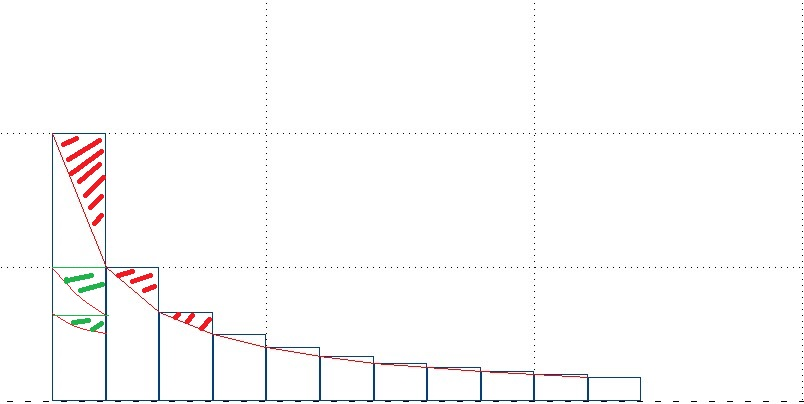
\includegraphics[width=10cm]{courbe.jpg}
    \caption{\(f(x)=\frac{1}{x}\) }
    \label{fig:fonction 1/x}
\end{figure}

Notons  \(p_1,p_2,...,p_n\)  les aires en rouge au dessus de la courbe, montrons que leur somme (notée \(S_n\)) correspond à la différence \(H_n - ln(n)\).
L'aire de chaque rectangle est simplement \(A_k = \frac{1}{x}*1\), l'aire sous la courbe est donnée par : \( I_k = \int_{k-1}^k \frac{1}{x} dx = ln(k)-ln(k-1) \).\\
Donc, \(p_k\) est égale à \(p_k = A_k - I_k = \frac{1}{k} - (ln(k)-ln(k-1))\), on a ensuite  \(S_n = \sum_{k=1}^n p_k= \sum_{k=1}^n (\frac{1}{k} - (ln(k)-ln(k-1)))\).
Après un léger calcul on a que \(S_n = H_n -ln(n) \).\\
On remarque que les aires rouge colorées sauf les n premiers s'emboîtent sans chevauchement dans le n + 1-ième rectangle d'aire 1/n. En d'autres termes, la somme des \(p_k\) converge et sa limite est \(\gamma\)  qui vérifie \(0 < \gamma-[H_n -ln(n)] \).\\
De plus, on observe qu'on peut translater toutes les aires rouge  dans le premier rectangle (aire translatée en vert) d'aire 1 sans chevauchement si bien qu'on a alors \(0<\gamma<1\). 


\subsection{Encadrement de $\gamma$ par la méthode des trapèzes}

\textbf{Rappel } : Si \( f \in \mathscr{C}^{2}([a,b]) \), alors il existe \( c \in ]a,b[ \) tel que :
\[
\int_{a}^{b} f(t)\,dt = \frac{b-a}{2} \big(f(a) + f(b)\big) - \frac{(b-a)^3}{12} f^{\prime\prime}(c).
\]

Il est bon d'observer que \( \frac{b-a}{2} \big(f(a) + f(b)\big) \) représente l'aire du trapèze

On en déduit la majoration de l'erreur dans la méthode des trapèzes :
\[
\left| \int_{a}^{b} f(t)\,dt - \frac{b-a}{2} \big(f(a) + f(b)\big) \right| \leq \frac{(b-a)^3}{12} \sup_{x \in [a,b]} |f^{\prime\prime}(x)|.
\]

\textbf{Preuve du rappel : } Par intégration par parties :

\[
\int_{a}^{b}\left(t-\frac{a+b}{2}\right)f^{\prime}(t)dt = \frac{b-a}{2}\cdot(f(a)+ f(b)) - \int_{a}^{b}f(t)dt
\]

Pour évaluer $\int_{a}^{b}\left(t-\frac{a+b}{2}\right)f^{\prime}(t)dt$ on fait encore une intégration par parties en choisissant cette fois $p(t)=-(b-t)(t-a)/2$ comme primitive de $t-\frac{a+b}{2}$ (c'est un polynôme de degré 2 s'annulant en $a$ et $b$ ce qui fera disparaître le terme « entre crochets »).

\[
\int_{a}^{b}\left(t-\frac{a+b}{2}\right)f^{\prime}(t)dt = \left[f^{\prime}(t)p(t)\right]_{a}^{b} - \int_{a}^{b}f^{\prime\prime}(t)p(t)dt = \frac{1}{2}\int_{a}^{b}f^{\prime\prime}(t)(b-t)(t-a)dt. \quad (14)
\]

Le polynôme $(b-t)(t-a)$ étant positif sur $[a,b]$ :

\[
\inf_{[a,b]}f^{\prime\prime}\int_{a}^{b}(b-t)(t-a)dt \leq \int_{a}^{b}f^{\prime\prime}(t)(b-t)(t-a)dt \leq \sup_{[a,b]}f^{\prime\prime}\int_{a}^{b}(b-t)(t-a)dt
\]

si bien que par le théorème des valeurs intermédiaires ($f^{\prime\prime}$ est continue) il existe $a<c<b$ vérifiant

\[
\int_{a}^{b}f^{\prime\prime}(t)(b-t)(t-a)dt = f^{\prime\prime}(c)\int_{a}^{b}(b-t)(t-a)dt
\]

soit finalement

\[
\int_{a}^{b}\left(t-\frac{a+b}{2}\right)f^{\prime}(t)dt = \frac{f^{\prime\prime}(c)}{2}\int_{a}^{b}(b-t)(t-a)dt = \frac{f^{\prime\prime}(c)}{12}(b-a)^{3}.
\]



(C'est en fait la formule de la moyenne pondérée). En reportant cette expression dans l'égalité initiale obtenue par intégration par parties, on obtient :

\[
\frac{f^{\prime\prime}(c)}{12}(b-a)^3 = \frac{b-a}{2}\big(f(a)+f(b)\big) - \int_{a}^{b}f(t)dt
\]

En réarrangeant les termes, on déduit la formule du trapèze avec reste intégral :

\[
\int_{a}^{b}f(t)dt = \frac{b-a}{2}\big(f(a)+f(b)\big) - \frac{f^{\prime\prime}(c)}{12}(b-a)^3
\]  \\ 



En appliquant la formule des trapèzes avec \( a = k - 1 \), \( b = k \) et \( f(t) = \dfrac{1}{t} \). Pour tout \( k \geq 2 \), il existe \( \zeta_k \in ]k-1,k[ \) tel que :
\[
\int_{k-1}^k \frac{\mathrm{d}t}{t} = \frac{1}{2} \left( \frac{1}{k} + \frac{1}{k-1} \right) - \frac{1}{6\zeta_k^3}.
\]

En sommant cette égalité pour \( k = 2 \) à \( n \), on obtient :
\begin{align*}
\sum_{k=2}^n \int_{k-1}^k \frac{\mathrm{d}t}{t}&= \frac{1}{2} \sum_{k=2}^n \left( \frac{1}{k} + \frac{1}{k-1} \right) - \sum_{k=2}^n \frac{1}{6\zeta_k^3} \\
ln(n) &= \frac{1}{2} \left( H_n - 1 + H_{n-1} \right) - \frac{1}{6} \sum_{k=2}^n \frac{1}{\zeta_k^3} \\
&= H_n - \frac{1}{2} - \frac{1}{2n} - \frac{1}{6} \sum_{k=2}^n \frac{1}{\zeta_k^3},
\end{align*}

On en déduit finalement :
\[
H_n - ln(n) = \frac{1}{2} + \frac{1}{2n} + \frac{1}{6} \sum_{k=2}^n \frac{1}{\zeta_k^3}.
\]

Enfin, comme \( 0 < \frac{1}{\zeta_k^2} < \frac{1}{(k-1)^3} \), la série de terme général \( \frac{1}{\zeta_k^3} \) converge et par conséquent la suite de terme général \( H_n - \ln(n) \) converge et sa limite \( \gamma \) vérifie :

\[
\gamma = \lim_{n \to \infty} (H_n -ln(n)) = \lim_{n \to \infty} \left( \frac{1}{2} + \frac{1}{2n} + \frac{1}{6} \sum_{k=2}^n \frac{1}{\zeta_k^3} \right) = \frac{1}{2} + \frac{1}{6} \sum_{k=2}^\infty \frac{1}{\zeta_k^3}.
\] \\

Pour $f(t) = t^{-3}$ décroissante, on a pour tout $k \geq 2$ :
\[ \int_{k}^{k+1} \frac{dt}{t^3} < \frac{1}{k^3} <  \int_{k-1}^{k} \frac{dt}{t^3} < \frac{1}{(k-1)^3} < \int_{k-2}^{k-1} \frac{dt}{t^3} \]

En sommant à partir de n + 1, on obtient

\[ \int_{n+1}^{\infty} \frac{dt}{t^3} < \sum_{k=n+1}^\infty \frac{1}{k^3} <  \int_{n}^{\infty} \frac{dt}{t^3} < \sum_{k=n+1}^\infty\frac{1}{(k-1)^3} < \int_{n-1}^{\infty} \frac{dt}{t^3} \]

Sachant l'inégalité suivante :

\[
\sum_{k=n+1}^\infty \frac{1}{k^3} < \sum_{k=n+1}^\infty \frac{1}{\zeta_k^3} < \sum_{k=n+1}^\infty\frac{1}{(k-1)^3}
\]

On en conclu que :

\[ \int_{n+1}^{\infty} \frac{dt}{t^3} < \sum_{k=n+1}^\infty \frac{1}{\zeta_k^3} < \int_{n-1}^{\infty} \frac{dt}{t^3}
\]

On peut évaluer l'integrale impopre et obtenir :

\[
\frac{1}{12(n+1)^{2}} = \frac{1}{6} \int_{n+1}^{\infty} \frac{dt}{t^{3}} < \frac{1}{6} \sum_{k \geq n+1} \frac{1}{\zeta_k^{3}} < \frac{1}{6} \int_{n-1}^{\infty} \frac{dt}{t^{3}} = \frac{1}{12(n-1)^{2}}
\] \\

A partir de l'inégalité précédente, on peut arriver à :

\[
\frac{1}{2} + \frac{1}{6} \sum_{k=2}^{n} \frac{1}{k^{3}} + \frac{1}{12(n+1)^{2}} < \frac{1}{2} + \frac{1}{6} \sum_{k=2}^{n} \frac{1}{\zeta_k^{3}} + \frac{1}{6} \sum_{k \geq n+1} \frac{1}{\zeta_k^{3}} < \frac{1}{2} + \frac{1}{6} \sum_{k=2}^{n} \frac{1}{\zeta_k^{3}}+ \frac{1}{12(n-1)^{2}}
\]

On peut réecrire cela en :

\[ \frac{1}{2} + \frac{1}{6} (\sum_{k=1}^{\infty} \frac{1}{k^{3}}  - \sum_{k \geq n+1}\frac{1}{k^3} - 1 )+ \frac{1}{12(n+1)^{2}} < \gamma < \frac{1}{2} + \frac{1}{6}( \sum_{k=1}^{\infty} \frac{1}{k^{3}} - \sum_{k \geq n+1}\frac{1}{(k-1)^3}) + \frac{1}{12(n-1)^{2}}\]

En simplifiant, on obtient :

\[ 
\frac{\zeta(3) + 2}{6} < \gamma < \frac{\zeta(3)+3}{6}
\]

Sachant que la constante d'Apéry $\zeta(3) = \sum_{k \geq 1}\frac{1}{k^3} \approx 1,2$ , on obtient l'encadrement :

\[0,53 < \gamma < 0,7\]

\subsection{Formule d'Euler-Maclaurin}

    \textbf{Théorème 2 }(Euler-Maclaurin) : Soit une fonction f(x) suffisamment régulière sur l'intervalle [a,b] alors la somme :
        
           \[ \sum_{k=0}^{b} f(k)\]
       
        peut être approximée par l'intégrale correspondante plus des termes correctifs : 
        
            \[\sum_{k=0}^{b} f(k) = \int_a^b f(x)dx + \frac{f(a)+f(b)}{2} + \sum_{k=1}^{b} \frac{B_{2k}}{(2k)!}\left[f^{(2k-1)}(b) - f^{2k-1}(a)\right] + R_n\]
        
        où \( B_{2k} \) sont les nombres de Bernoulli pairs \\
        où \( f^{(2k-1)}(x)\)  désigne les dérivés successifs impairs de \( f(x)\) \\
        où \( Rn \) est un terme de reste qui dépend des dérivées de \( f \) \\\\

\textbf{Preuve :} On peut écrire :
        \[
        \sum_{k=a}^{b} f(k) = \sum_{k=a}^{b} \int_k^{k+1} f(k) \, dx = \sum_{k=a}^{b} \int_k^{k+1} f(x) \, dx + \sum_{k=a}^{b} \left(f(k) - \int_k^{k+1} f(x)\, dx\right).
        \]
        Le premier terme donne l’intégrale $\int_a^{b+1} f(x)\, dx$. On recentre ensuite sur $\int_a^b f(x)\, dx$.
        
        
        Ensuite, l’idée est de corriger l’intégrale $\int_a^b f(x)\, dx$ pour obtenir la somme $\sum_{k=a}^{b} f(k)$ à l’aide des polynômes de Bernoulli. On utilise l'identité suivante valable pour toute fonction $f \in C^{2m}$ :
        \[
        \int_a^b f(x)\, dx = \sum_{k=a}^{b-1} \int_k^{k+1} f(x)\, dx.
        \]
        Sur chaque intervalle $[k, k+1]$, on change de variable : $x = k + t$, avec $t \in [0,1]$. Alors :
        \[
        \int_k^{k+1} f(x)\, dx = \int_0^1 f(k + t)\, dt.
        \]
        On développe $f(k + t)$ en série de Taylor centrée en $k$ :
        \[
        f(k + t) = \sum_{n=0}^{2m-1} \frac{f^{(n)}(k)}{n!} t^n + \frac{f^{(2m)}(p)}{(2m)!} t^{2m}, \quad \text{avec } p \in (k, k+1).
        \]
        On intègre sur $t \in [0,1]$ :
        \[
        \int_0^1 f(k + t)\, dt = \sum_{n=0}^{2m-1} \frac{f^{(n)}(k)}{n!} \int_0^1 t^n dt + \frac{1}{(2m)!} \int_0^1 f^{(2m)}(p_t) t^{2m} dt.
        \]
        Mais $\int_0^1 t^n dt = \frac{1}{n+1}$, donc on peut réécrire :
        \[
        \int_0^1 f(k + t)\, dt = \sum_{n=0}^{2m-1} \frac{f^{(n)}(k)}{(n+1)n!} + R_k,
        \]
        où $R_k$ est le reste associé à $f^{(2m)}$.
        
        On compare cela à $f(k)$, en introduisant une identité classique :
        \[
        f(k) = \int_0^1 f(k)\, dt = \int_0^1 \left[f(k+t) - \sum_{r=1}^{m} \frac{B_{2r}(t)}{(2r)!} f^{(2r)}(k) \right] dt + \sum_{r=1}^{m} \frac{B_{2r}}{(2r)!} f^{(2r)}(k).
        \]
        
        En sommant sur $k = a, \ldots, b$, et en intégrant par parties les termes en $B_{2r}(t)$, on obtient les termes correctifs :
        \[
        \sum_{r=1}^{m} \frac{B_{2r}}{(2r)!} \left( f^{(2r-1)}(b) - f^{(2r-1)}(a) \right),
        \]
        plus un reste intégral :
        \[
        R_m = \frac{(-1)^{m+1}}{(2m)!} \int_a^b B_{2m}(x - \lfloor x \rfloor) f^{(2m)}(x) \, dx.
        \] \\\\


Si nous posons $f(x) = \frac{1}{x}$, la formule ci-dessus entraîne :

\[
1 + \frac{1}{2} + \cdots + \frac{1}{n} 
= \log n + \frac{1}{2} + \frac{1}{2n} + \frac{b_2}{2}\left(1 - \frac{1}{n^2}\right) + \cdots + \frac{b_{2k}}{2k}\left(1 - \frac{1}{n^{2k}}\right) - \int_1^n \frac{B_{2k+1}(\{x\})}{x^{2k+2}} \, dx.
\]

Quand $n \to +\infty$, on obtient

\[
\gamma = \frac{1}{2} + \frac{b_2}{2} + \cdots + \frac{b_{2k}}{2k} - \int_1^{+\infty} \frac{B_{2k+1}(\{x\})}{x^{2k+2}} \, dx.
\] \\

On peut utiliser cette formule pour approximer la valeur de $\gamma$ \\

- Terme intégrale:
  \[
  \int_1^n \frac{1}{x}dx = ln(n)
  \]

- Terme de correction avec \( f(a) \) et \( f(b) \) où a = 1 et b = n:
  \[
  \frac{1}{2} \left( 1 + \frac{1}{n}\right) = \frac{1}{2} + \frac{1}{2n}
  \]

- Terme correctif de Bernoulli : \\ \\
  Les nombres de Bernoulli sont :
  \[
  B_2 = \frac{1}{6}, \quad B_4 = \frac{-1}{30}, \quad B_6 = \frac{1}{42}, \quad \dots
  \]
  Les dérivées successives de \(f(x) = \frac{1}{x}\) sont :
  \[
  f^{(1)}(x) = \frac{-1}{x^2}, \quad f^{(3)}(x) = \frac{-6}{x^4}, \quad f^{(5)} = \frac{-120}{x^6}, \quad \dots
  \]
  Avec x = n, on obtient :
  \[
   \frac{B_2}{2!}\left(\frac{-1}{n^2} + 1 \right)\ = \frac{1}{12}\left(\frac{-1}{n^2} + 1 \right)\ = \frac{-1}{12n^2} + \frac{1}{12}
  \]
  \[
   \frac{B_4}{4!}\left(\frac{-6}{n^4} + 6\right)\ = \frac{-1}{720}\left(\frac{-6}{n^4} + 2 \right)\ = \frac{1}{120n^4} - \frac{1}{120}
  \]
  \[
   etc\dots
  \]
 
On obtient alors : 
  \[
   H_n = ln(n) + \frac{1}{2} + \frac{1}{2n} + \frac{-1}{12n^2} + \frac{1}{12} + \frac{1}{120n^4} - \frac{1}{120} + \mathcal{O}(\frac{1}{n^6})
  \]
 \\
En soustrayant le logarithme et en passant a la limite, on obtient :
 \[
\lim\limits_{n \to \infty}( {H_n} - ln(n)) = \frac{1}{2} + \frac{1}{12} - \frac{1}{120} \approx 0.575
  \]

  Ce qui en fait une approximation intéressante de $\gamma$
        

        

\subsection{Approximation par un algorithme}

L'algorithme suivant permet de calculer une approximation de la constante d'Euler en sommant les inverses des entiers et en soustrayant $\ln n$.

\begin{itemize}
    \item \textbf{Entrées :} $N > 1$
    \item \textbf{Initialisation :} $U \gets 0$
    \item \textbf{Traitement :} pour $I$ de $1$ à $N$, ajouter $\frac{1}{I}$ à $U$ puis soustraire $\ln N$
    \item \textbf{Sortie :} Afficher $U$
\end{itemize}

\[
U = \sum_{I=1}^N \frac{1}{I} - ln N
\]

La convergence de la suite $(u_n)$ est relativement lente. Voici un tableau montrant les valeurs de $u_n$ pour différentes valeurs de $N$ :

\[
\begin{array}{|c|c|}
\hline
N & u_N \\
\hline
10 & 0.6264 \\
50 & 0.5872 \\
200 & 0.5797 \\
500 & 0.5782 \\
1000 & 0.5777 \\
2000 & 0.5775 \\
5000 & 0.5773 \\
\hline
\end{array}
\]

Après 5000 itérations, la précision est encore limitée à 3 décimales.


On observe que même en augmentant \( n \) de façon significative, la valeur de \( H_n \) ne croît que très lentement.


\newpage
\section{Résultats et formules impliquant $\gamma$}

\subsection{$\gamma$ et des intégrales}

\textbf{Proposition 9 :} \\
\[
\gamma=\int_{0}^{\infty}e^{-t}\left(\frac{1}{1-e^{-t}}-\frac{1}{t}\right)dt= \int_{0}^{1}\left(\frac{1}{1-t}+\frac{1}{ln(t)}\right)dt.
\] \\

\textbf{Preuve :}
Commençons par montrer que \ln(n) = $\int_0^\infty \frac{e^{-t}-e^{-nt}}{t} dt&. 
\[
\begin{align*}
ln(n) = \int_1^n \frac{dr}{r} = \int_1^n \left( \int_0^\infty e^{-rt} dt \right) dr = \int_0^\infty \left( \int_1^n \, e^{-rt} dr \right) dt = \int_0^\infty \frac{e^{-t}-e^{-nt}}{t} dt.
\end{align*}
\]

Les égalités précédentes nous permettent d'écrire
\[
H_{n}-ln(n) =\sum_{k=1}^{n}\int_{0}^{\infty}e^{-kt}dt-\int_{0}^{\infty}\frac{e^{-t}-e^{-nt}}{t}dt=\int_{0}^{\infty}e^{-t}\frac{1-e^{-nt}}{1-e^{-t}}dt-\int_{0}^{\infty}\frac{e^{-t}-e^{-nt}}{t}dt
\]
\[
=\int_{0}^{\infty}\left(e^{-t}\frac{1-e^{-nt}}{1-e^{-t}}-\frac{e^{-t}-e^{-nt}}{t}\right)dt
\]
\[
=\int_{0}^{\infty}\left(e^{-t}\left(\frac{1}{1-e^{-t}}-\frac{1}{t}\right)+e^{-nt}\left(\frac{1}{t}-\frac{e^{-t}}{1-e^{-t}}\right)\right)dt
\]
\[
=\int_{0}^{\infty}e^{-t}\left(\frac{1}{1-e^{-t}}-\frac{1}{t}\right)dt+\int_{0}^{\infty}e^{-nt}\left(\frac{1}{t}-\frac{1}{e^{t}-1}\right)dt
\]
car les deux dernières intégrales convergent (utilisez les DL pour obtenir des équivalents en \(0\) et \(+\infty\)).

3. (3) Si on passe à la limite dans l'égalité précédente, il vient
\[
\gamma=\lim_{n \to \infty}(H_{n}-ln(n))=\int_{0}^{\infty}e^{-t}\left(\frac{1}{1-e^{-t}}-\frac{1}{t}\right)dt+\lim_{n \to \infty}\int_{0}^{\infty}e^{-nt}\left(\frac{1}{t}-\frac{1}{e^{t}-1}\right)dt.
\]
Il s'agit donc de prouver que \(\lim_{n}\int_{0}^{\infty}e^{-nt}\left(\frac{1}{t}-\frac{1}{e^{t}-1}\right)dt=0\), autrement dit que la limite peut rentrer dans l'intégrale ce que l'on va justifier par convergence dominée. Vu que pour tout \(t\in\mathbb{R}_+^* : e^{t}\geq 1+t\) assure \(\frac{1}{e^{t}-1}\leq\frac{1}{t}\), on a la domination valable pour tout \(x>0\) et \(n\geq 1 : |e^{-nt}\left(\frac{1}{t}-\frac{1}{e^{t}-1}\right)|\leq e^{-t}\left|\frac{1}{t}-\frac{1}{1-e^{-t}}\right|\). L'échange
\[
\lim_{n}\int_{0}^{\infty}e^{-nt}\left(\frac{1}{t}-\frac{1}{e^{t}-1}\right)dt= \int_{0}^{\infty}\lim_{n}e^{-nt}\left(\frac{1}{t}-\frac{1}{e^{t}-1}\right)dt=0
\]
Enfin le changement de variable \(v=e^{-t}\) dans \(\int_{0}^{\infty}e^{-t}\left(\frac{1}{1-e^{-t}}-\frac{1}{t}\right)dt\) donne finalement
\[
\gamma=\int_{0}^{\infty}e^{-t}\left(\frac{1}{1-e^{-t}}-\frac{1}{t}\right)dt= \int_{0}^{1}\left(\frac{1}{1-t}+\frac{1}{ln(t)}\right)dt.
\]

\subsection{$\gamma$ et la fonction $\zeta$ de Riemann}

\textbf{Proposition 10 :} \[
\gamma = \lim_{x\to 1^+} \sum_{n=1}^\infty \left(\frac{1}{n^x} - \frac{1}{x^n}\right) = \lim_{x\to 1^+} \left(\zeta(x) - \frac{1}{x-1}\right)
\] \\

\textbf{Preuve : }Nous avons : 

\[
\gamma = \lim_{n} H_{n} - ln(n+1)
\]

(car \(\lim_{n\to\infty} ln(n) - ln(n+1) = \lim_{n} ln\left(\frac{n}{n+1}\right) = 0\)) et

\[
ln(n+1) = \int_{1}^{n+1} \frac{dt}{t} = \sum_{k=1}^{n} \int_{k}^{k+1} \frac{dt}{t}.
\]

D'un autre côté, pour \(x > 1\), on peut écrire :

\[
\sum_{n=1}^{\infty} \frac{1}{x^{n}} = \frac{1}{x-1} = \int_{1}^{\infty} \frac{dt}{t^{x}} = \sum_{n=1}^{\infty} \int_{n}^{n+1} \frac{dt}{t^{x}}.
\]

En réunissant tout cela nous avons :

\[
\gamma = \lim_{n\to\infty} \left(H_{n} - ln(n+1)\right) = \lim_{n\to\infty} \left(\sum_{k=1}^{n} \frac{1}{k} - \int_{k}^{k+1} \frac{dt}{t}\right)
\]
\[
= \lim_{n\to\infty} \sum_{k=1}^{n} \left(\frac{1}{k} - \int_{k}^{k+1} \frac{dt}{t}\right) = \sum_{k=1}^{\infty} \left(\frac{1}{k} - \int_{k}^{k+1} \frac{dt}{t}\right)
\]
\[
= \sum_{k=1}^{\infty} \lim_{x\to 1_{+}} \left(\frac{1}{k^{x}} - \int_{k}^{k+1} \frac{dt}{t^{x}}\right) =_{(1)} \lim_{n \to \infty} \sum_{k= 1}^{\infty} \left(\frac{1}{k^{x}} - \int_{k}^{k+1} \frac{dt}{t^{x}}\right)
\]
\[
= \lim_{x\to 1_{+}} \left(\sum_{k=1}^{\infty} \frac{1}{k^{x}} - \sum_{k=1}^{\infty} \int_{k}^{k+1} \frac{dt}{t^{x}}\right) = \lim_{x\to 1_{+}} \left(\sum_{k=1}^{\infty} \frac{1}{k^{x}} - \sum_{k=1}^{\infty} \frac{1}{x^{k}}\right)
\]

Ce qu'il nous fallait démontrer. Il reste tout de même à justifier l'échange limite/somme (1). Pour cela, si on pose \(f_{k}(x) = \frac{1}{k^{x}} - \int_{k}^{k+1} \frac{dt}{t^{x}}\) et \(F(x) = \sum_{k} f_{k}(x)\) alors (1) équivaut à \(F(1) = \lim_{x\to 1_{+}} F(x)\) ; il est donc suffisant de prouver la convergence uniforme de la série de fonctions.(continues) $\sum_{k}\,f_{k}$ sur $[1,2]$ pour conclure avec le théorème de Weierstrass. Pour $x\in[1,2]:$

\[
|f_{k}(x)| = \frac{1}{k^{x}} - \int_{k}^{k+1}\frac{dt}{t^{x}} = \int_{k}^{k+1} \left(\frac{1}{k^{x}} - \frac{1}{t^{x}}\right)dt
\]
\[
= \int_{k}^{k+1}\left(\int_{k}^{t}\frac{x}{u^{x+1}}du\right)dt \leq \int_{k}^{k+1}\left(\int_{k}^{t}\frac{x}{k^{x+1}}du\right)dt
\]
\[
= \frac{x}{k^{x+1}}\int_{k}^{k+1}(t-k)dt = \frac{x}{2k^{x+1}} \leq \frac{1}{k^{2}}.
\]

Ainsi $\sup_{x\in[1,2]}|f_{k}(x)| \leq \frac{1}{k^{2}}$ d'où la convergence uniforme sur $[1,2]$ de notre série de fonctions, d'où la continuité en $x=1_{+}$ de $F$ d'où (1). \\ \\

\subsection{Apparition de $\gamma$ dans l'expression de la fonction $\psi$(x)}
 \color{black}

\textbf{Proposition 11 : } Pour x appartenant à  $\mathbb{R}_+^\ast$, 

\[ \psi(x) = \frac{\Gamma'(x)}{\Gamma(x)} = - \gamma + \sum_{n=1}^\infty [\frac{1}{n+x} - \frac{1}{n}]\]

On va d'abord démontrer cela, 
en utilisant le produit de Weierstrass :
\[
\frac{1}{\Gamma(x)} = x e^{\gamma x} \prod_{n=1}^{\infty} \left(1 + \frac{x}{n}\right) e^{-x/n}
\]


Prenons le logarithme naturel des deux côtés de l'égalité du produit de Weierstrass :
\[
ln\left(\frac{1}{\Gamma(x)}\right) = ln\left(x e^{\gamma x} \prod_{n=1}^{\infty} \left(1 + \frac{x}{n}\right) e^{-x/n}\right)
\]
\[
-ln(\Gamma(x)) = ln(x) + ln(e^{\gamma x}) + ln\left(\prod_{n=1}^{\infty} \left(1 + \frac{x}{n}\right) e^{-x/n}\right)
\]
\[
-ln(\Gamma(x)) = ln(x) + \gamma x + \sum_{n=1}^{\infty} ln\left(\left(1 + \frac{x}{n}\right) e^{-x/n}\right)
\]
\[
-ln(\Gamma(x)) = ln(x) + \gamma x + \sum_{n=1}^{\infty} \left[ ln\left(1 + \frac{x}{n}\right) + ln\left(e^{-x/n}\right) \right]
\]
\[  
-ln(\Gamma(x)) = ln(x) + \gamma x + \sum_{n=1}^{\infty} \left[ ln\left(1 + \frac{x}{n}\right) - \frac{x}{n} \right]
\]


En dérivant, on a : \begin{align*}
(-ln(\Gamma(x)))' &= \frac{1}{x} + \gamma + \sum_{n=1}^{\infty} \left[ \frac{1}{1 + \frac{x}{n}} \cdot \frac{1}{n} - \frac{1}{n} \right] \\
& = -\frac{\Gamma'(x)}{\Gamma(x)} = -\psi(x) \\
& = \frac{1}{x} + \gamma + \sum_{n=1}^{\infty} \left[ \frac{n}{n+x} \cdot \frac{1}{n} - \frac{1}{n} \right] \\
& = \frac{1}{x} + \gamma + \sum_{n=1}^{\infty} \left[ \frac{1}{n+x} - \frac{1}{n} \right]
\end{align*} avec \[(-ln(\Gamma(x)))' =  -\frac{\Gamma'(x)}{\Gamma(x)} = -\psi(x)\]

donc \[\psi(x) = -\frac{1}{x} - \gamma - \sum_{n=1}^{\infty} \left[ \frac{1}{n+x} - \frac{1}{n} \right]\] \\


  

\subsection{Constante d'Euler et constante d'Euler}

\textbf{Proposition 12 :}
Pour un entier positif \( n \), soit \( g_n = 1 + \frac{1}{2} + \cdots + \frac{1}{n} - ln n \).

\[
\lim_{n \to \infty} \left( \frac{g_n^\gamma}{\gamma^{g_n}} \right)^{2n} = \frac{e}{\gamma},
\]

\textbf{Preuve :}
La formule d'Euler-Maclaurin explorée plus tôt donne l'estimation bien connue

\[
g_n = 1 + \frac{1}{2} + \cdots + \frac{1}{n} - \ln n = \gamma + \frac{1}{2n} + O \left( \frac{1}{n^2} \right).
\]

Ainsi, \( g_n = \gamma + \epsilon_n \), où \( \epsilon_n = \frac{1}{2n} + O \left( \frac{1}{n^2} \right) \) et \( 2n\epsilon_n = 1 + O \left( \frac{1}{n} \right) \). On a alors

\[
\left( \frac{g_n^y}{\gamma^{g_n}} \right)^{2n} = \left( \frac{(\gamma + \epsilon_n)^\gamma}{\gamma^{\gamma+\epsilon_n}} \right)^{2n} = \frac{\left( 1 + \frac{2n\epsilon_n}{2\gamma n} \right)^{2\gamma n}}{\gamma^{2n\epsilon_n}} = \frac{\left( 1 + \frac{1+O\left( \frac{1}{n} \right)}{2 \gamma n} \right)^{2 \gamma n}}{\gamma^{1+O\left( \frac{1}{n} \right)}}.
\]

Comme

\[
\lim_{n \to \infty} \left( 1 + \frac{1 + O \left( \frac{1}{n} \right)}{2\gamma n} \right)^{2 \gamma n} = \lim_{n \to \infty} \left( 1 + \frac{1}{2 \gamma n} \right)^{2 \gamma n} = e \quad \text{et} \quad \lim_{n \to \infty} \gamma^{1+O\left( \frac{1}{n} \right)} = \gamma,
\]

le résultat suit.


\subsection{Une inégalité intéressante}

\textbf{Proposition 13 : }Pour tous \(m,n\ge1\),
\[
\gamma \;<\; H_m + H_n - H_{mn} \;<\; 1,
\]
où \(H_k=\sum_{j=1}^k\frac1j\) et \(\gamma=\lim_{p\to\infty}(H_p - \ln p)\).

\medskip

On écrit tout d’abord
\[
H_m + H_n - H_{mn}
= (H_m + H_n - H_n)
  - (H_{2n}-H_n) - (H_{3n}-H_{2n}) - \cdots - (H_{mn}-H_{(m-1)n})
\]
soit, en regroupant,
\[
H_m + H_n - H_{mn}
= H_m
  - \sum_{k=1}^{m-1}\bigl(H_{kn} - H_{(k-1)n}\bigr)
= H_m
  - \sum_{k=1}^{m-1}\sum_{j=(k-1)n+1}^{kn}\frac1j.
\]
Or, pour chaque \(k=1,\dots,m-1\),
\[
\sum_{j=(k-1)n+1}^{kn}\frac1j
\;\ge\;
n\cdot\frac1{kn}
=\frac1k.
\]
D’où
\[
H_m + H_n - H_{mn}
\;\le\;
H_m - \sum_{k=1}^{m-1}\frac1k
=1.
\]

Pour l’inégalité inférieure, on utilise que la suite \(H_p - \ln p\) décroît vers \(\gamma\).  
En posant \(p=nm\) et \(p=n\), on obtient
\[
\gamma < H_{nm} - ln(nm) < H_n - ln n
\;\Longrightarrow\;
0 < H_n - ln n - H_{nm} + ln(nm).
\]
Comme on a par ailleurs \(\gamma < H_m - ln m\), la somme de ces deux inégalités donne
\[
\gamma
< \bigl(H_m - ln m\bigr)
  + \bigl(H_n - ln n - H_{nm} + ln(nm)\bigr)
= H_m + H_n - H_{mn}.
\]

\newpage

\section*{Conclusion}

La constante d’Euler-Mascheroni \(\gamma\) demeure aujourd’hui une énigme mathématique fascinante, à la croisée de plusieurs disciplines : analyse, théorie des nombres, probabilités, algorithmique. Son apparition naturelle dans l’étude des séries harmoniques et des fonctions spéciales comme \(\Gamma\) ou \(\zeta\) témoigne de sa profonde richesse théorique.

Bien que définie de manière élémentaire comme la différence entre une somme partielle harmonique et un logarithme, \(\gamma\) révèle une complexité étonnante. Malgré les siècles de recherche, des questions aussi fondamentales que son irrationalité ou sa transcendance restent ouvertes, ce qui confère à cette constante un statut à part dans le paysage mathématique.

Les approches analytiques, les méthodes d’intégration, les transformations via la fonction \(\Gamma\) ou encore les estimations numériques ont permis de mieux cerner ses propriétés, mais non de percer tous ses mystères. Cette constante illustre ainsi l’un des traits les plus profonds des mathématiques : la simplicité apparente d’un objet peut cacher une complexité insoupçonnée.

En somme, \(\gamma\) n’est pas seulement une constante parmi d’autres ; elle est un point de convergence entre intuition arithmétique et rigueur analytique, un symbole de l’incomplétude actuelle de nos connaissances et un appel constant à l’exploration mathématique.


\section*{Bibliographie}

\begin{enumerate}[label={[{\bfseries \arabic*}]}]

\item \url{https://www.methodemaths.fr/}

\item P. Lassere, \textit{Autour de $\gamma$, la constante d’Euler.}

\item \url{https://www.lyceedadultes.fr/sitepedagogique/documents/math/mathTermS/02_raisonnement_recurrence_limite_suite/02_cours_constante_euler.pdf}

\item \url{https://agreg-maths.fr/uploads/versions/5381/Formule%20d'Euler%20Maclaurin.pdf}

\item \url{https://fr.wikipedia.org/wiki/Formule_d%27Euler-Maclaurin}

\item Sur le calcul numérique de la constante d’Euler
Gazette des Mathématiciens, vol. 27, (1985), p. 113–126 

\item \url{https://www.lyceedadultes.fr/sitepedagogique/documents/math/mathTermS/02_raisonnement_recurrence_limite_suite/02_cours_constante_euler.pdf}

\item \url{https://www.bibmath.net/dico/index.php?action=affiche&quoi=./e/eulercst.html}

\end{enumerate}
\end{document}







